\section{Front-end}
	\subsection{SPA}
	
		 Web sẽ thiết kế theo kiểu Single Page Application (SPA) thay vì theo kiểu truyền thống là Server side rendering. Ưu điểm của cách thiết kế này là web sẽ có trải nghiệm như khi dùng ứng dụng trên điện thoại hoặc máy tính. Mỗi lần thực hiện một thao tác hay chuyển trang trên web thì trình duyệt sẽ không phải load lại trang nữa. Việc này được thực hiện bằng cách sử dụng AJAX để lấy dữ liệu một cách bất đồng bộ từ phía server mỗi khi có một event do người dùng thực hiện trên trình duyệt. Sau đó, ta sẽ sử dụng dữ liệu lấy được (Thường là dưới dạng JSON) để đổ giao diện lên trình duyệt hiển thị cho người dùng.
    
	\subsection{ReactJS}
	
		\begin{figure}[!ht]
			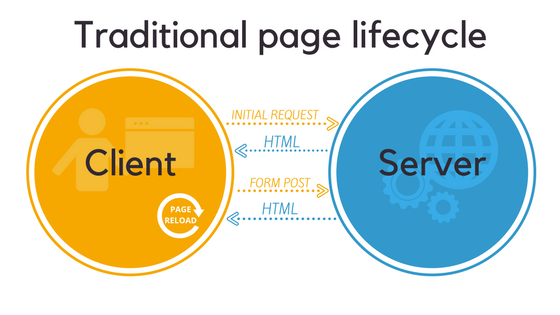
\includegraphics[width=0.8\textwidth]{/MPA.png}
			\centering
			\linebreak
			\caption{Luồng dữ liệu của các trang web MPA truyền thống}
		\end{figure}
	
		\begin{figure}[!ht]
			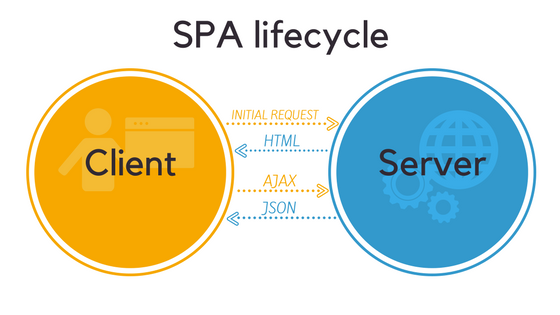
\includegraphics[width=0.8\textwidth]{/SPA.png}
			\centering
			\linebreak
			\caption{Luồng dữ liệu của các trang web SPA}
		\end{figure}
	
		\textbf{ReacJS} được phát triển bởi Facebook là một thư viện rất phổ biến để phát triển các ứng dụng web SPA hiện nay. React Cho phép người lập trình có thể chia ứng dụng thành các component và tái sử dụng, nhờ vậy mà tiết kiệm được thời gian lập trình. Hơn nữa, cơ chế DOM ảo \textbf{(Virtual DOM)} mới chính là điểm đặc biệt hơn cả của thư viện ReactJS. Cập nhật cây DOM là một tác vụ khá tốn chi phí. Nếu như để lập trình một cách thông thường, lập trình viên tự quản lí DOM bằng các Native API của môi trường web thì sẽ dễ gây ra vấn đề về hiệu suất. Chính vì vậy ReactJS sẽ giúp ta cập nhật DOM bằng cách quản lí ngầm một cây DOM ảo và sẽ đối chiếu những thay đổi so với các phiên bản DOM ảo trước đó để cập nhật lên cây DOM thật, giúp ứng dụng web tăng hiệu suất. Chính vì những lí do trên mà nhóm quyết định sẽ sử dụng thư viện này để phát triển luận văn này.\\
		
		\begin{figure}[!ht]
			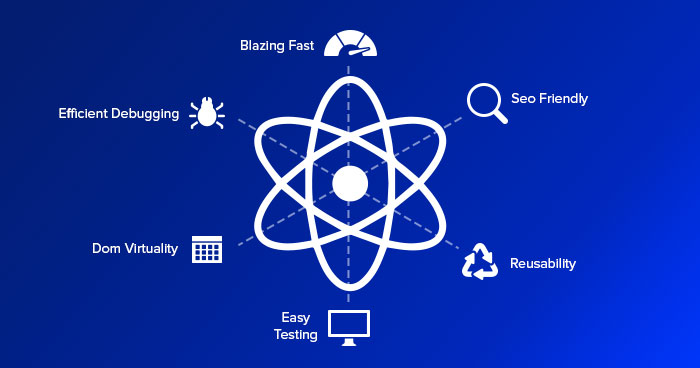
\includegraphics[width=0.8\textwidth]{/ReactJS.jpg}
			\centering
			\linebreak
			\caption{ReactJS và những lợi ích khi sử dụng}
		\end{figure}
		
		Bên cạnh đó, ReactJS cho phép người lập trình có thể viết bằng 2 ngôn ngữ: Javascript và Typescript. Javascript đã ra đời và được sử dụng từ rất lâu. Hiện nay, đây là ngôn ngữ được rất nhiều lập trình viên sử dụng, cả trong việc phát triển ứng dụng phía client-side lẫn phía server-side. JS là một ngôn ngữ prototype-based hỗ trợ cả lập trình hướng đối tượng và lập trình hàm, các tính năng được bảo trì và phát triển liên tục. Tuy vậy, quá linh động cũng là một điểm yếu của ngôn ngữ này. JS không kiểm tra ràng buộc kiểu khi chúng ta viết mã nguồn. Người lập trình có thể sử dụng một biến mà không cần khai báo kiểu, khiến cho việc truyền tham số hay khi tương tác các biến khác kiểu trở nên khó kiểm soát. Lấy ví dụ đơn giản như biểu thức "1" + 1 sẽ là hợp lệ và không bị bắt lỗi trong quá trình kiểm tra kiểu tĩnh khi chúng ta lập trình. Hay khi ta định nghĩa một hàm với các tham số cần truyền vào, do JS không hỗ trợ khai báo kiểu nên khi gọi hàm ta có thể truyền bất cứ tham số với bất cứ kiểu nào, làm cho hàm có thể thực thi ngoài ý muốn. Chính vì vậy, TypeScript ra đời để giải quyết vấn đề của JS kể trên. TypeScript yêu cầu người dùng định nghĩa kiểu rõ ràng cho các biến, kiểu trả về của hàm và bắt lỗi các biểu thức mà có sự tương tác của các biến không tương thích kiểu. Nhờ vậy, Sử dụng TS sẽ giúp cho mã nguồn của dự án dễ đọc, minh bạch, dễ bảo trì và phát triển hơn rất nhiều.
		
		\begin{figure}[!ht]
			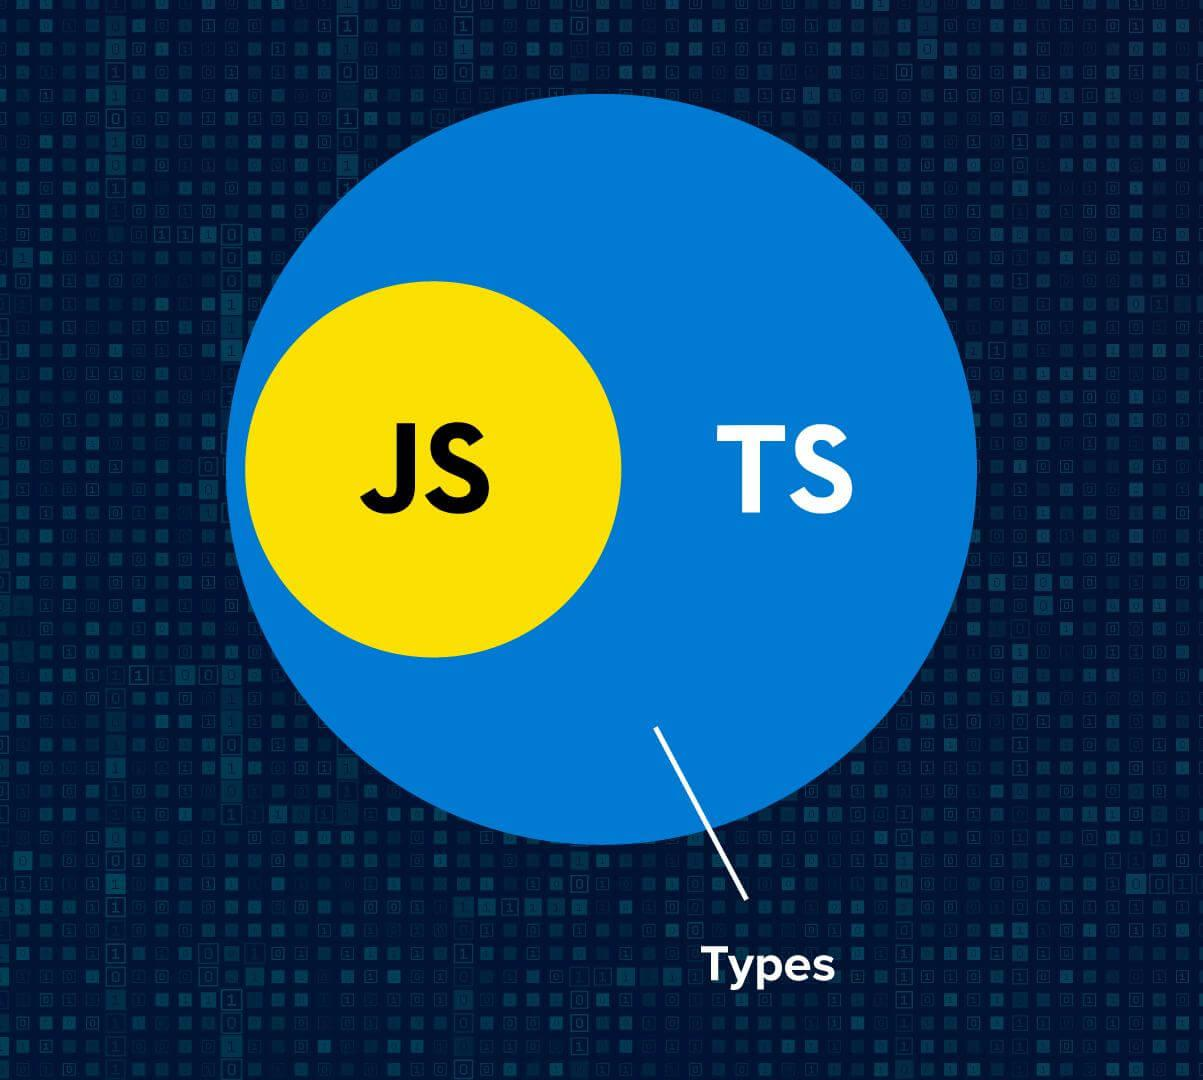
\includegraphics[width=0.8\textwidth]{/TypeScript.jpg}
			\centering
			\linebreak
			\caption{TypeScript là phiên bản mở rộng của JS có hỗ trợ kiểm tra kiểu tĩnh}
		\end{figure}
	
        \subsection{Continuous integration / Continuous deployment (CI/CD)}	
		Do web SPA sẽ trả về file html tĩnh cho người dùng tương tác (Dữ liệu hiển thị được cập nhật bằng cách tương tác với API phía server) nên ta có thể host website trên những dịch vụ cho host static web miễn phí. Nhóm sẽ chọn dịch vụ host web tĩnh miễn phí của gitlab để làm môi trường test (staging). Ưu điểm của gitlab là vừa có thể giúp nhóm quản lí source code cũng như cung cấp dịch vụ Continuous integration (CI) và continuous delivery (CD) giúp có thể deploy ứng dụng một cách tự động mỗi khi ta push code lên gitlab.\\
		
		Cụ thể, CI/CD giúp chúng ta chỉ phải code, chia branch đẩy lên git. Các công đoạn như unit test, deployment sẽ được gitlab-runner thực hiện một cách tự động mỗi khi có thay đổi mã nguồn. Bất kì ứng dụng được phát triển hiện nay đều cần phải qua khâu Unit Test do chính người lập trình viết trước khi được chuyển qua cho bộ phận kiểm thử phần mềm. Khi ta đẩy mã nguồn lên git mà quên chạy lệnh để kiểm thử unit test ở dưới máy local thì gitlab-runner sẽ giúp nhóm lập trình chạy các test case đó và sẽ thông báo trên giao diện git nếu có test case bị fail. Sau giai đoạn chạy các unit test và đã qua hết các test case thì tất nhiên, ứng dụng phải được deploy lên các môi trường (staging, production, etc). Việc phải SSH vào server host ứng dụng, sau đó tải mã nguồn mới nhất về, build ứng dụng ra các file tối ưu để chạy là khá tốn thời gian. Các thao tác trên thực chất cũng chỉ là chạy các câu lệnh trên terminal, vậy tại sao không để hệ thống tự động chạy những câu lệnh đó? Ta chỉ cần liệt kê các câu lệnh của một hành động cần phải thực hiện theo đúng thứ tự và hệ thống CI/CD của gitlab sẽ tự động chạy các câu lệnh đó cho chúng ta.
		
		\begin{figure}[!ht]
1			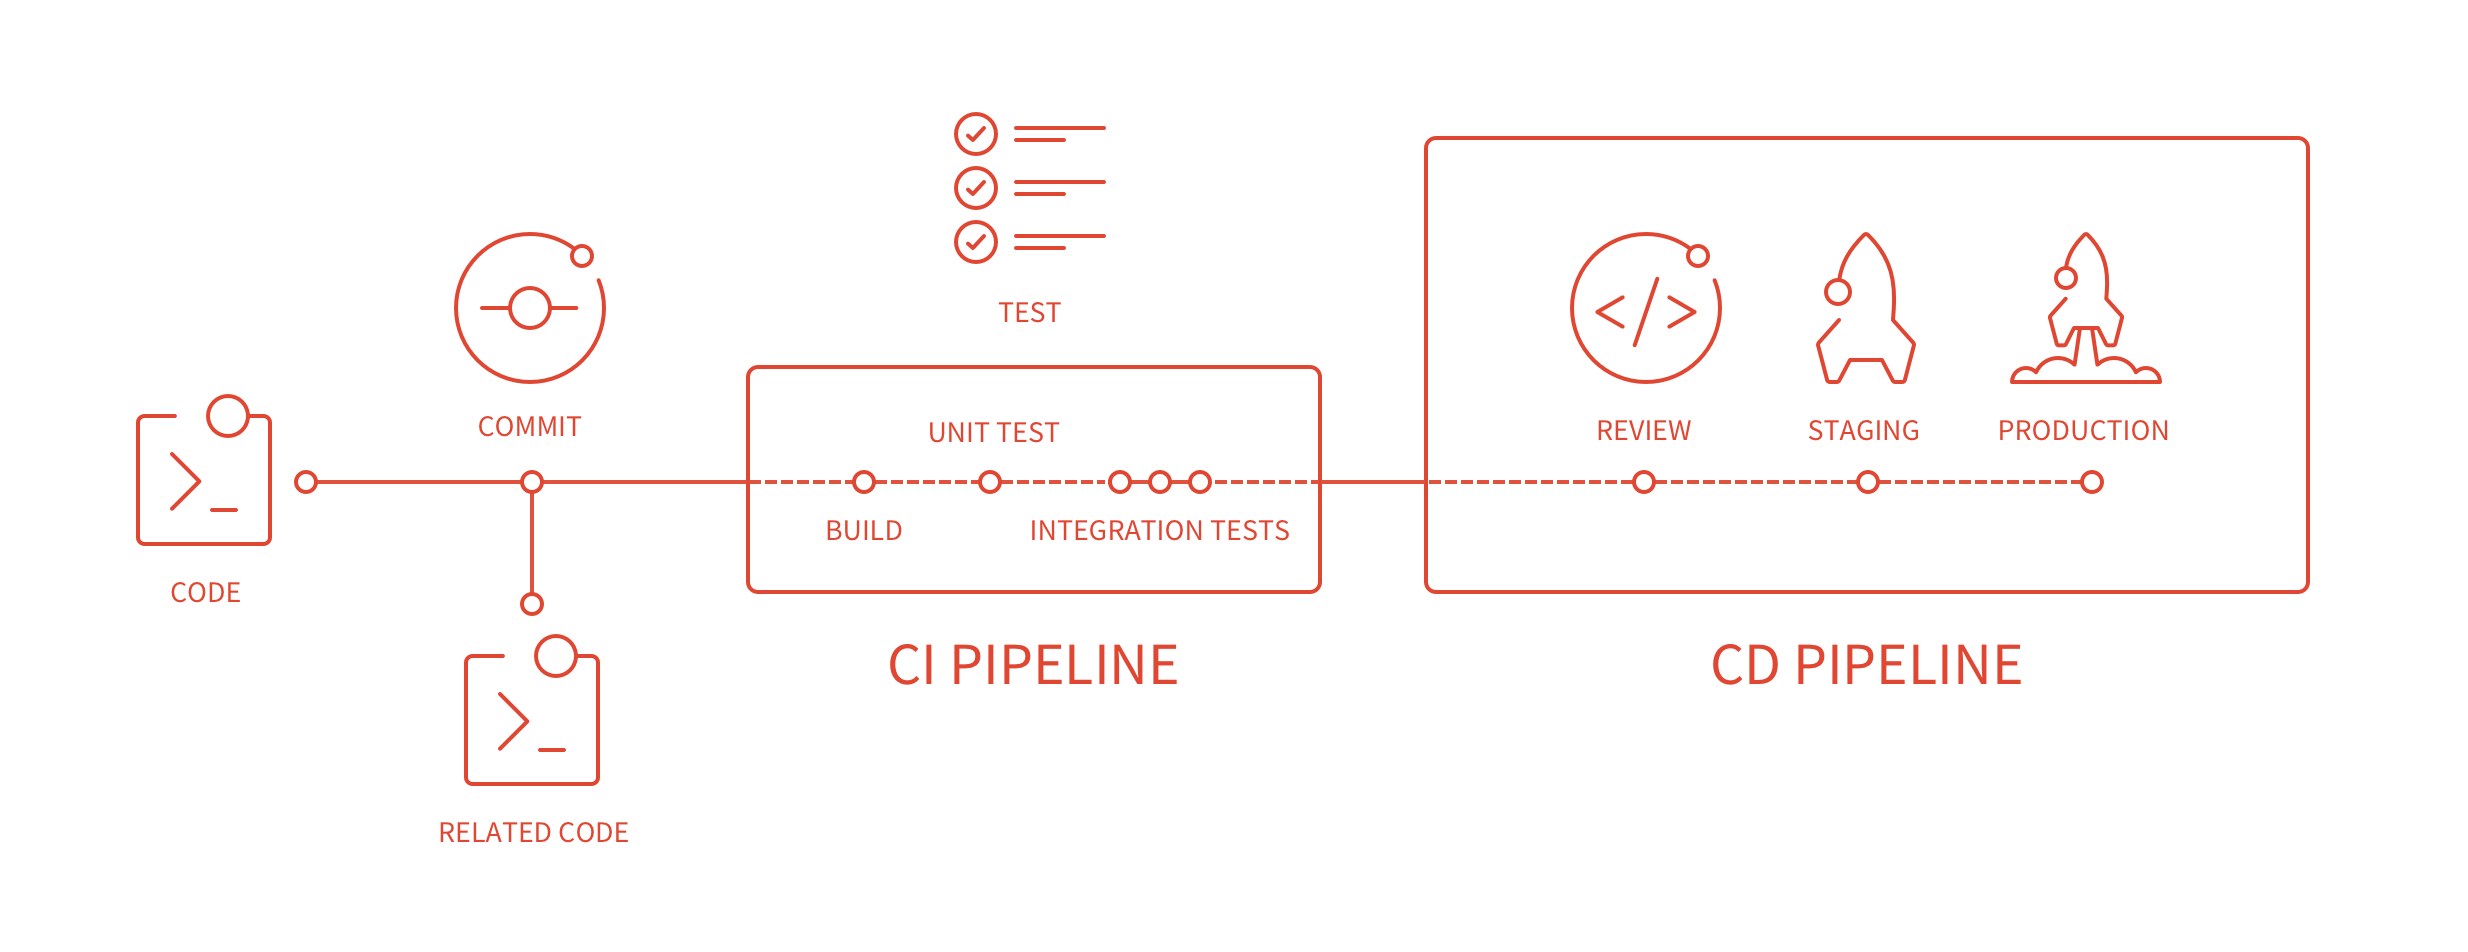
\includegraphics[width=1\textwidth]{/cicd.png}
			\centering
			\linebreak
			\caption{Gitlab CICD}
		\end{figure}
	
		\subsection{Những thư viện nổi bật giúp hiện thực chức năng hệ thống}
			Một số lập trình viên rất thích việc xây dựng mọi thứ từ đầu và hạn chế sử dụng thư viện càng nhiều càng tốt. Tuy vậy, có những tính năng đã được một số thư viện hỗ trợ đầy đủ và đã được kiểm thử qua hàng ngàn người dùng. Khi đó, ta nên sử dụng thư viện để tiết kiệm thời gian phát triển cũng như có thể sử dụng ngay lập tức tính năng chất lượng đã qua kiểm thử. Nhóm sẽ liệt kê một số thư viện nổi bật (Ngoài thư viện chính React) mà nhóm đã dùng để hiện thực một vài chức năng của hệ thống: \\
			
			Nhóm sẽ giới thiệu một số thư viện được áp dụng trong việc viết code phía client mà nhóm thấy nổi bật để trình bày:\\
			
			\begin{itemize}
				\item \textbf{chart.js (version 2.9.4):} Dùng để hiện thực chức năng tạo biểu đồ thống kê của admin.
				\item \textbf{date-fns (version 2.21.1):} Dùng để thực hiện việc tính toán ngày tháng như lấy thời gian bắt đầu / kết thúc của ngày, tăng giảm số ngày vv...
				\item \textbf{antd (version 4.9.4):} Thư viện CSS và component tương thích với React.
				\item \textbf{json-bigint (version 1.0.0):} Giúp parse ra được ID lớn của đơn hàng thành chuỗi dạng string.
				\item \textbf{@react-pdf/renderer (version 2.0.8):} Giúp tạo ra template cho phiếu nhập/xuất kho dưới dạng pdf.
				\item \textbf{gzipper (version 4.5.0):} Giúp tạo ra những file gzip của những file static đã build ra. Như vậy sẽ giảm dung lượng đường truyền mạng cần thiết để tải file và trang web sẽ hiển thị nhanh hơn vào lần đầu tiên truy cập.
			\end{itemize}
			
	
		\subsection{Giám sát lỗi hệ thống bằng dịch vụ Sentry}
			\subsubsection{Giới thiệu về Sentry}
				Một hệ thống không những phải hoạt động tốt mà còn cần phải có hệ thống ghi log và báo cáo lỗi không mong muốn xảy ra từ người dùng. Thay vì phải tự hiện thực lại hệ thống như trên thì nhóm đã quyết định sử dụng một dịch vụ trực tuyến khá phổ biến và nổi tiếng hiện nay: Sentry. Về cơ bản. Sentry giúp chúng ta theo dõi lại những lỗi xảy ra bên trong ứng dụng trong quá trình người dùng sử dụng. Thông thường khi lỗi xảy ra, người dùng sẽ có xu hướng tắt ứng dụng và mở lại chứ không report lại cho bên phía đội ngũ phát triển. Sentry sẽ tự động gửi report chi tiết về lỗi đó một cách tự động và nhanh chóng. Giúp cho người lập trình có thể nhanh chóng cập nhật bản vá sửa lỗi đó trước khi nhiều người dùng bị lỗi tương tự.
				
			\subsubsection{Áp dụng sentry cho hệ thống giao hàng liên tỉnh}
			 	Nhận thấy tác dụng hữu ích và đồng thời muốn học thêm những công nghệ đang thịnh hành ngoài thị trường. Nhóm chúng em đã thử áp dụng Sentry vào hệ thống giao hàng liên tỉnh này. Sau đây là một số kết quả mà nhóm đã thu được từ việc áp dụng Sentry:
			 	
			 	\begin{figure}[H]
			 		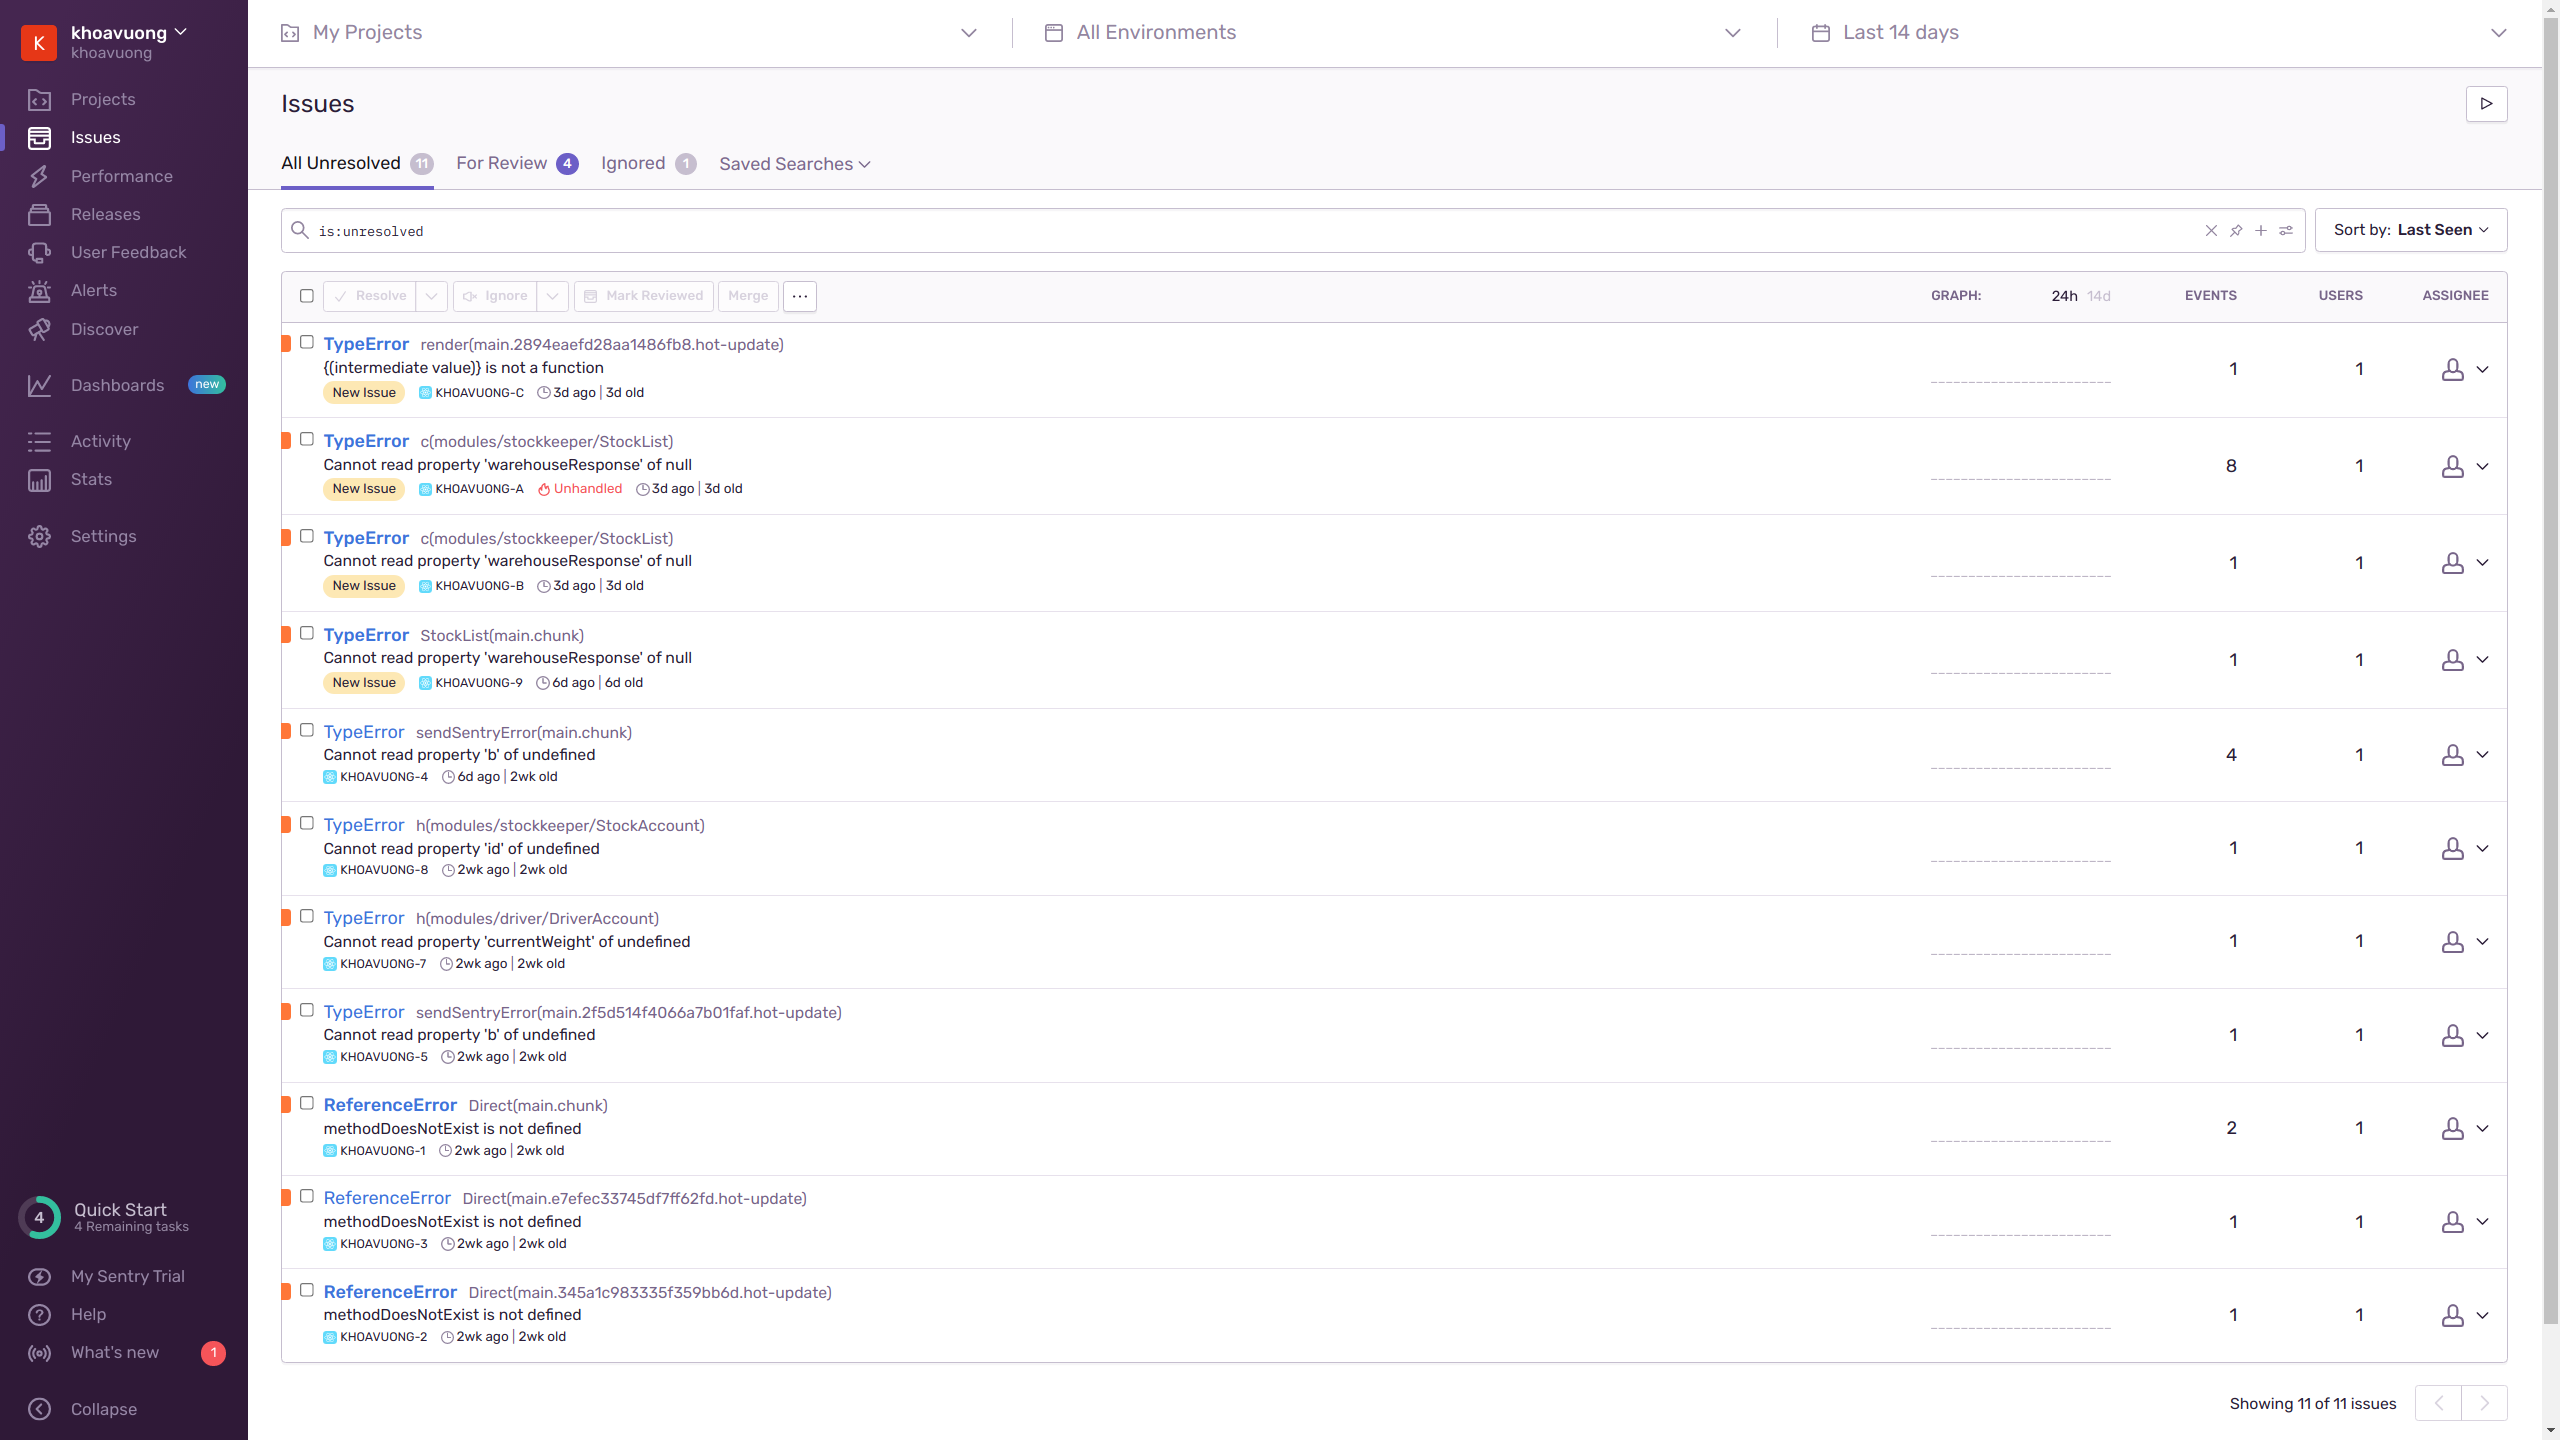
\includegraphics[width=0.8\textwidth]{/sentry/sentry_dashboard.png}
			 		\centering
			 		\caption{Giao diện dashboard để xem những lỗi được gửi về}
			 	\end{figure}
		 	
		 		Có thể thấy giao diện trên liệt kê ra những lỗi chưa được xử lý của ứng dụng khi người dùng tương tác. Ở giao diện dashboard đó ta có thể chọn một hoặc nhiều lỗi được gửi về và đánh dấu đã xử lí (Resolve) sau khi đã thực hiện bản vá sửa lỗi hoặc bỏ qua (Ignore) nếu như lỗi đó không cần phải giải quyết. Những lỗi đã được xử lí sẽ bị mất đi trong danh sách lỗi ở màn hình dashboard đó. \\
		 		
		 		Ngoài ra, khi click vào liên kết của một lỗi cụ thể. Sentry sẽ đưa ta đến một giao diện để xem một cách chi tiết thông tin về lỗi đó:
		 		
			 	\begin{figure}[H]
			 		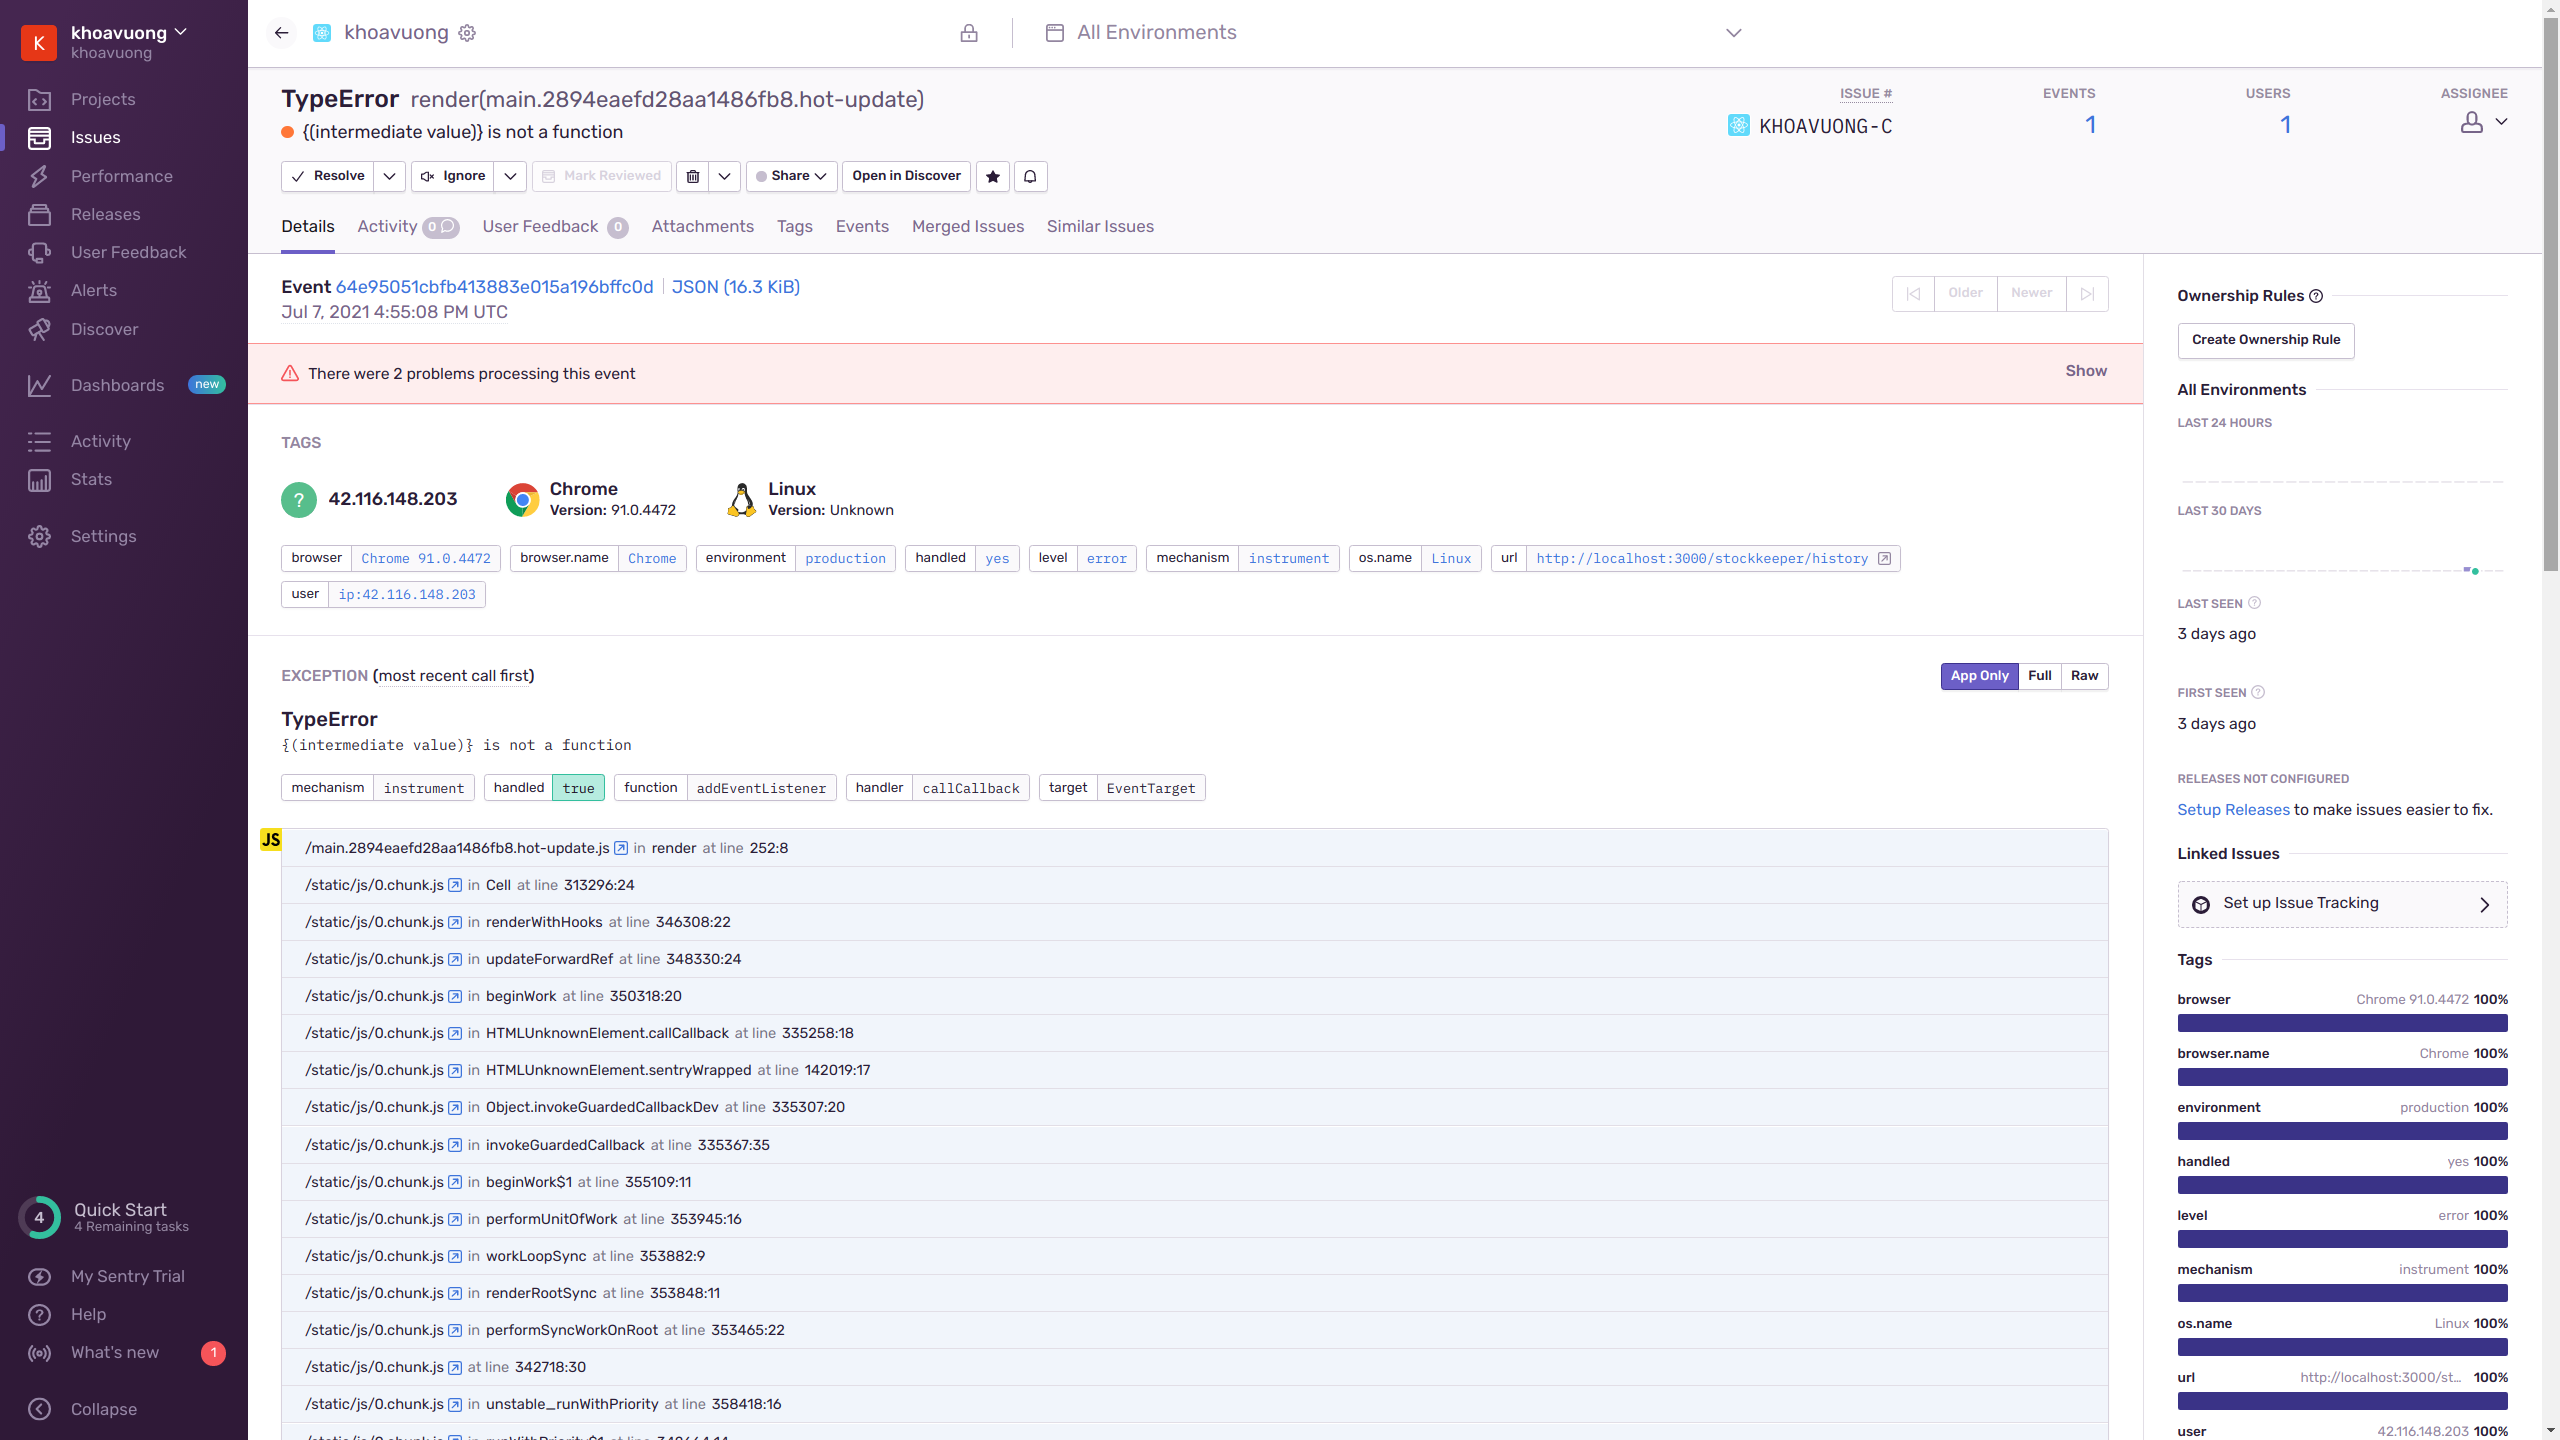
\includegraphics[width=0.8\textwidth]{/sentry/sentry_detail_1.png}
			 		\centering
			 		\caption{Giao diện xem lỗi gửi về chi tiết (Nửa trên màn hình)}
			 	\end{figure}
		 	
		 		\begin{figure}[H]
		 			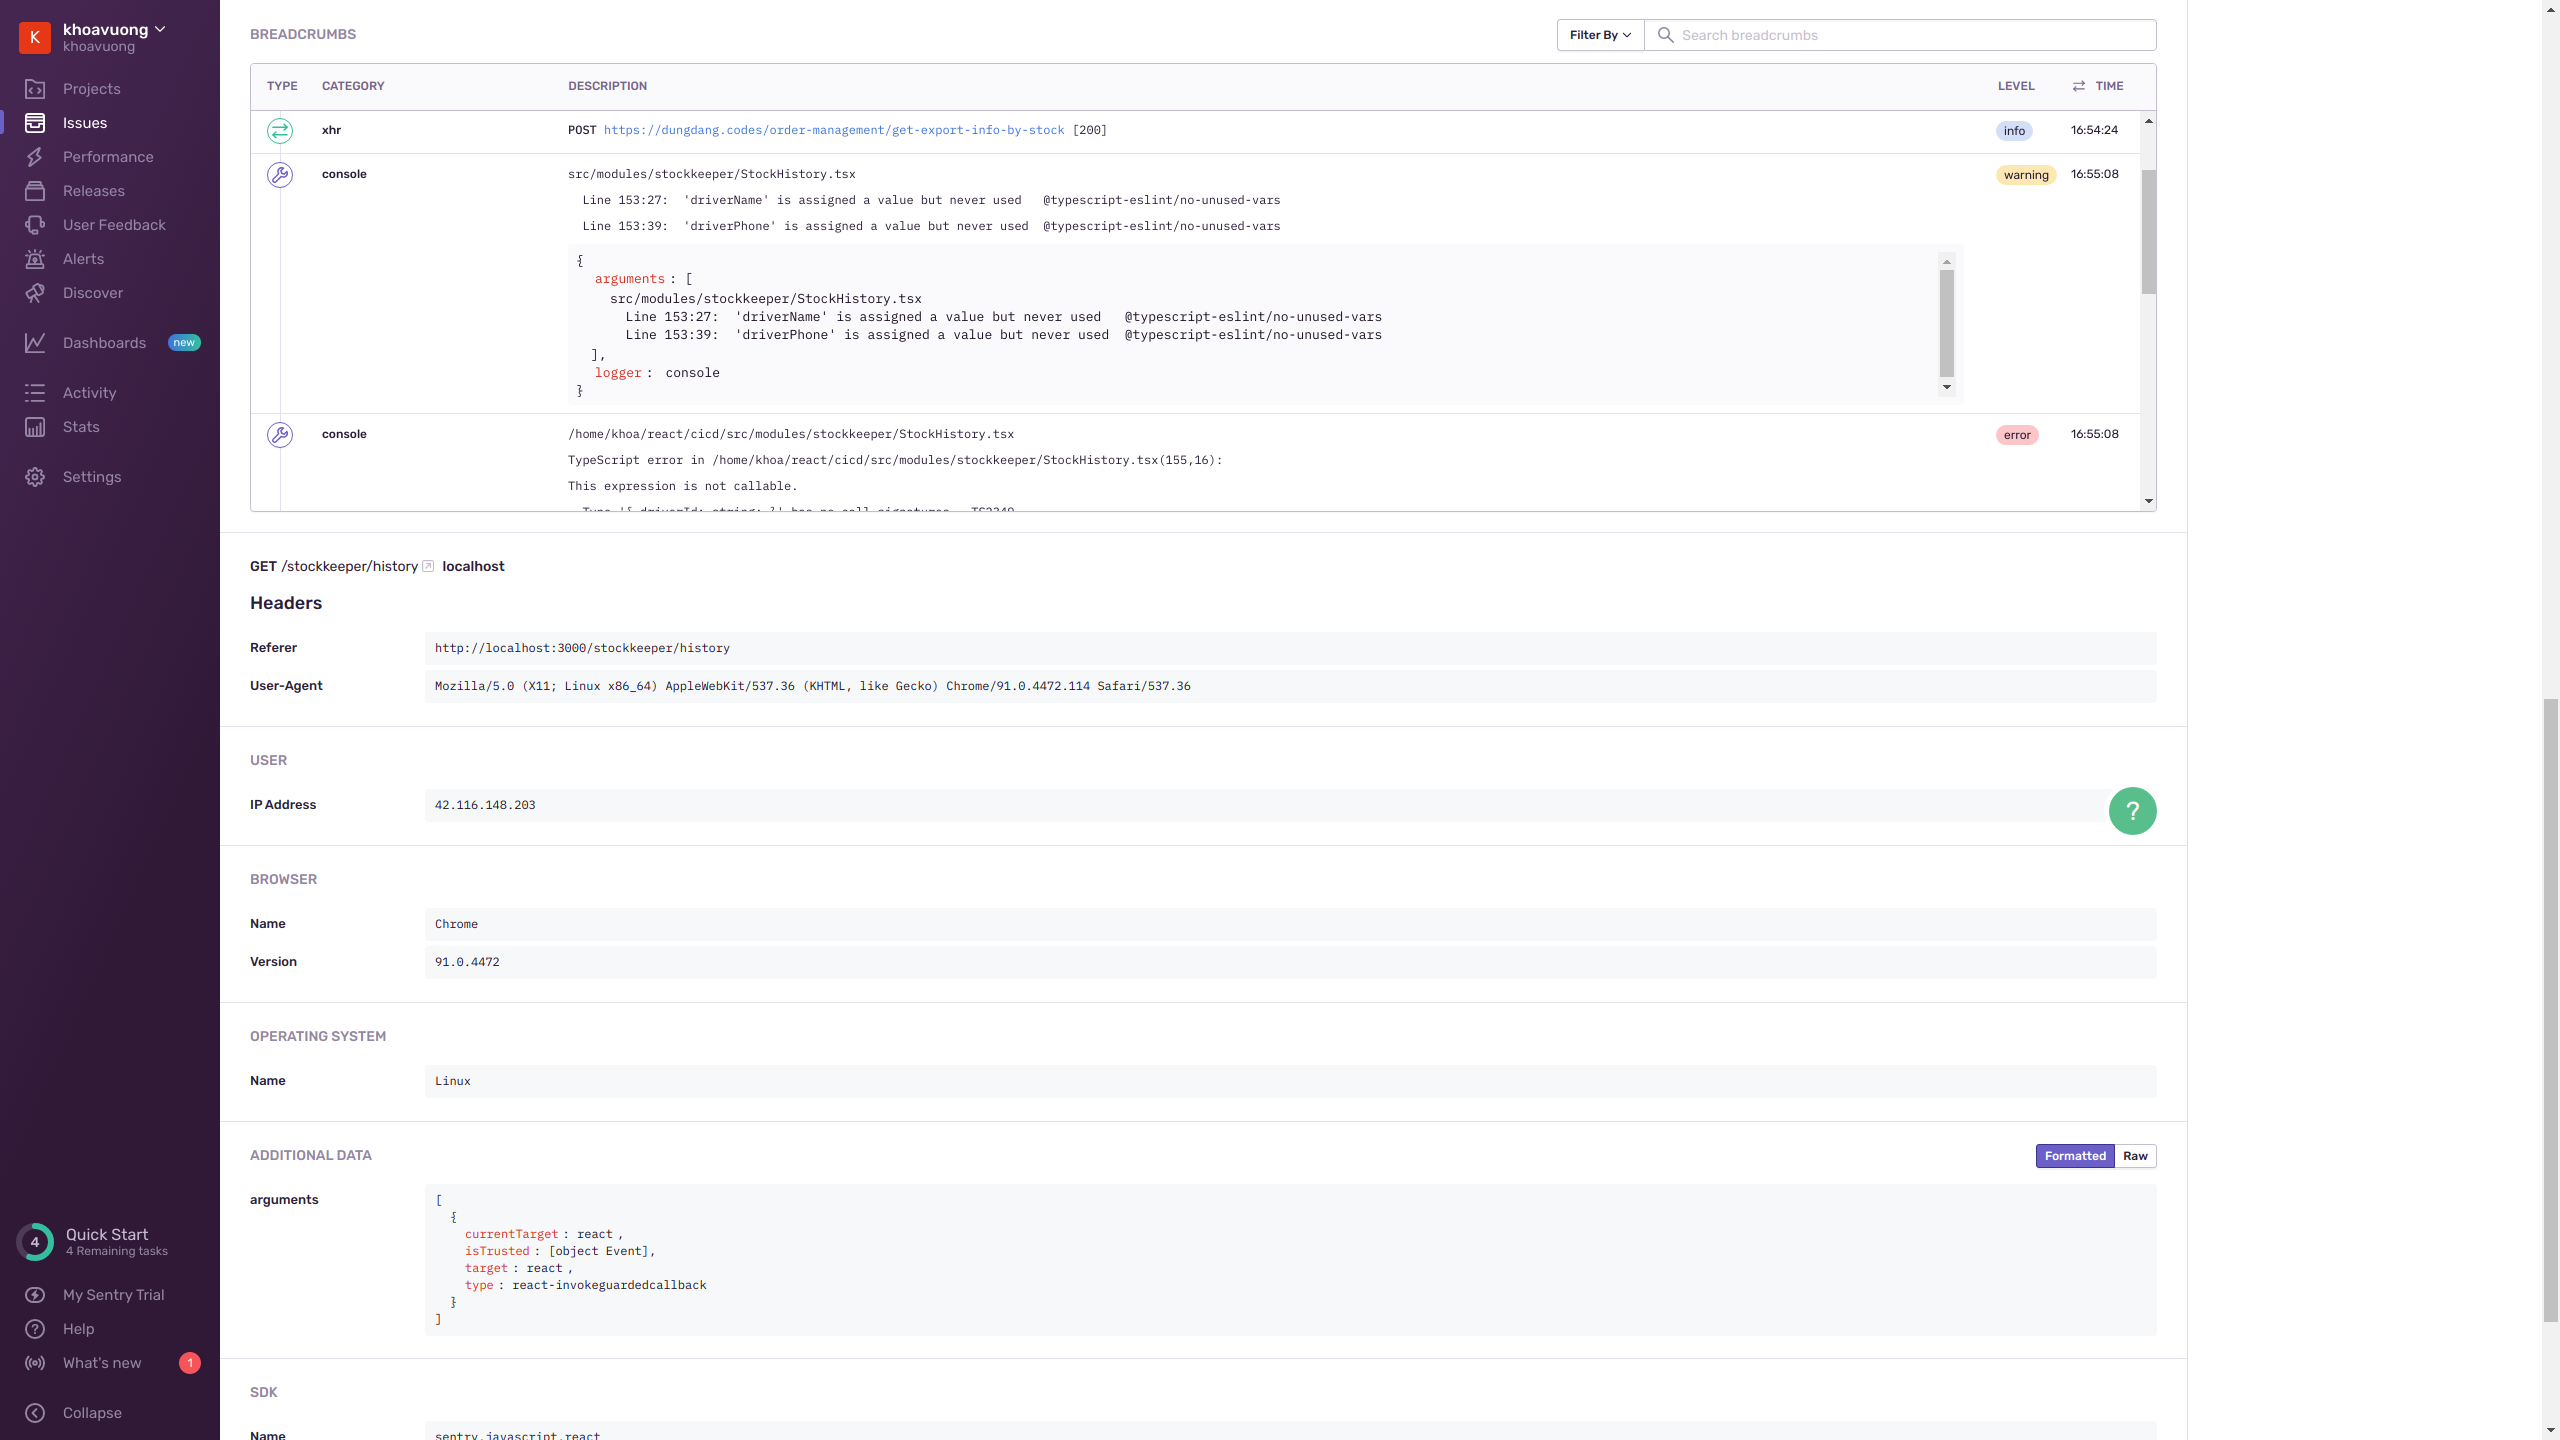
\includegraphics[width=0.8\textwidth]{/sentry/sentry_detail_2.png}
		 			\centering
		 			\caption{Giao diện xem lỗi gửi về chi tiết (Nửa dưới màn hình)}
		 		\end{figure}
			 	
			 	Giao diện đó cung cấp cho người lập trình toàn bộ thông tin quan trọng để có thể bắt đầu việc debug và sửa lỗi. Có thể kể đến một số thông tin hữu ích như ngày xảy ra lỗi, trình duyệt web, địa chỉ IP, OS của người dùng. Không những thế, Sentry còn liệt kê cho ta chi tiết lỗi xảy ra ở đoạn mã lệnh nào giúp cho người lập trình dễ dàng phát hiện đoạn mã lỗi để sửa. Ở ví dụ cụ thể trong hình trên. Ta có thể thấy được lỗi xảy ra tại địa chỉ IP 42.116.148.203, trình duyệt web Chrome và hệ điều hành Linux. Đoạn lệnh lỗi cũng được chỉ ra nằm ở tập tin nào và nguyên nhân xảy ra lỗi. \\
			 	
			 	Tóm tắt lại, Sentry là một nền tảng rất phổ biến hiện nay giúp cho hệ thống chúng ta xây dựng có thể nhanh chóng phát hiện lỗi từ phía người dùng. Hầu như mọi dự án lớn đều đang sử dụng Sentry và hiệu quả nó mang lại là không phải bàn cãi.
			 	
			 	\subsection{Phân tích số lượng và hành vi người dùng với Google Analytics}
			 	Một website không chỉ cần có hệ thống giám sát lỗi không mong muốn từ người dùng mà cũng cần phải có một hệ thống dùng để thống kê, theo dõi lưu lượng truy cập và những tương tác của người dùng với trang web. Từ đó đội ngũ phát triển có thể đưa ra những quyết định và những bản cập nhật để phục vụ nhu cầu người dùng tốt hơn. Cũng tương tự như trên, thay vì phải tốn thời gian và công sức xây dựng hệ thống đó thì nhóm cũng quyết định sử dụng một dịch vụ thống kê rất phổ biến và được ưa chuộng hiện nay: Google Analytics. Đây là một dịch vụ được cung cấp miễn phí bởi Google.
			 	
			 	\subsubsection{Áp dụng Google Analytics vào hệ thống}
			 	Nhận thấy đây là công nghệ rất phổ biến và hữu dụng. Nhóm đã quyết định sử dụng Google Analytics vào để có thể xem được chi tiết những thống kê người dùng truy cập đến trang web. Đây cũng là một cơ hội để học hỏi thêm một công nghệ mới được sử dụng bởi nhiều doanh nghiệp.\\
			 	
			 	Sau đây là một số tính năng theo dõi và thống kê thời gian thực của người dùng của website do Google Analytics đã thu thập:
			 	
			 	\begin{figure}[H]
			 		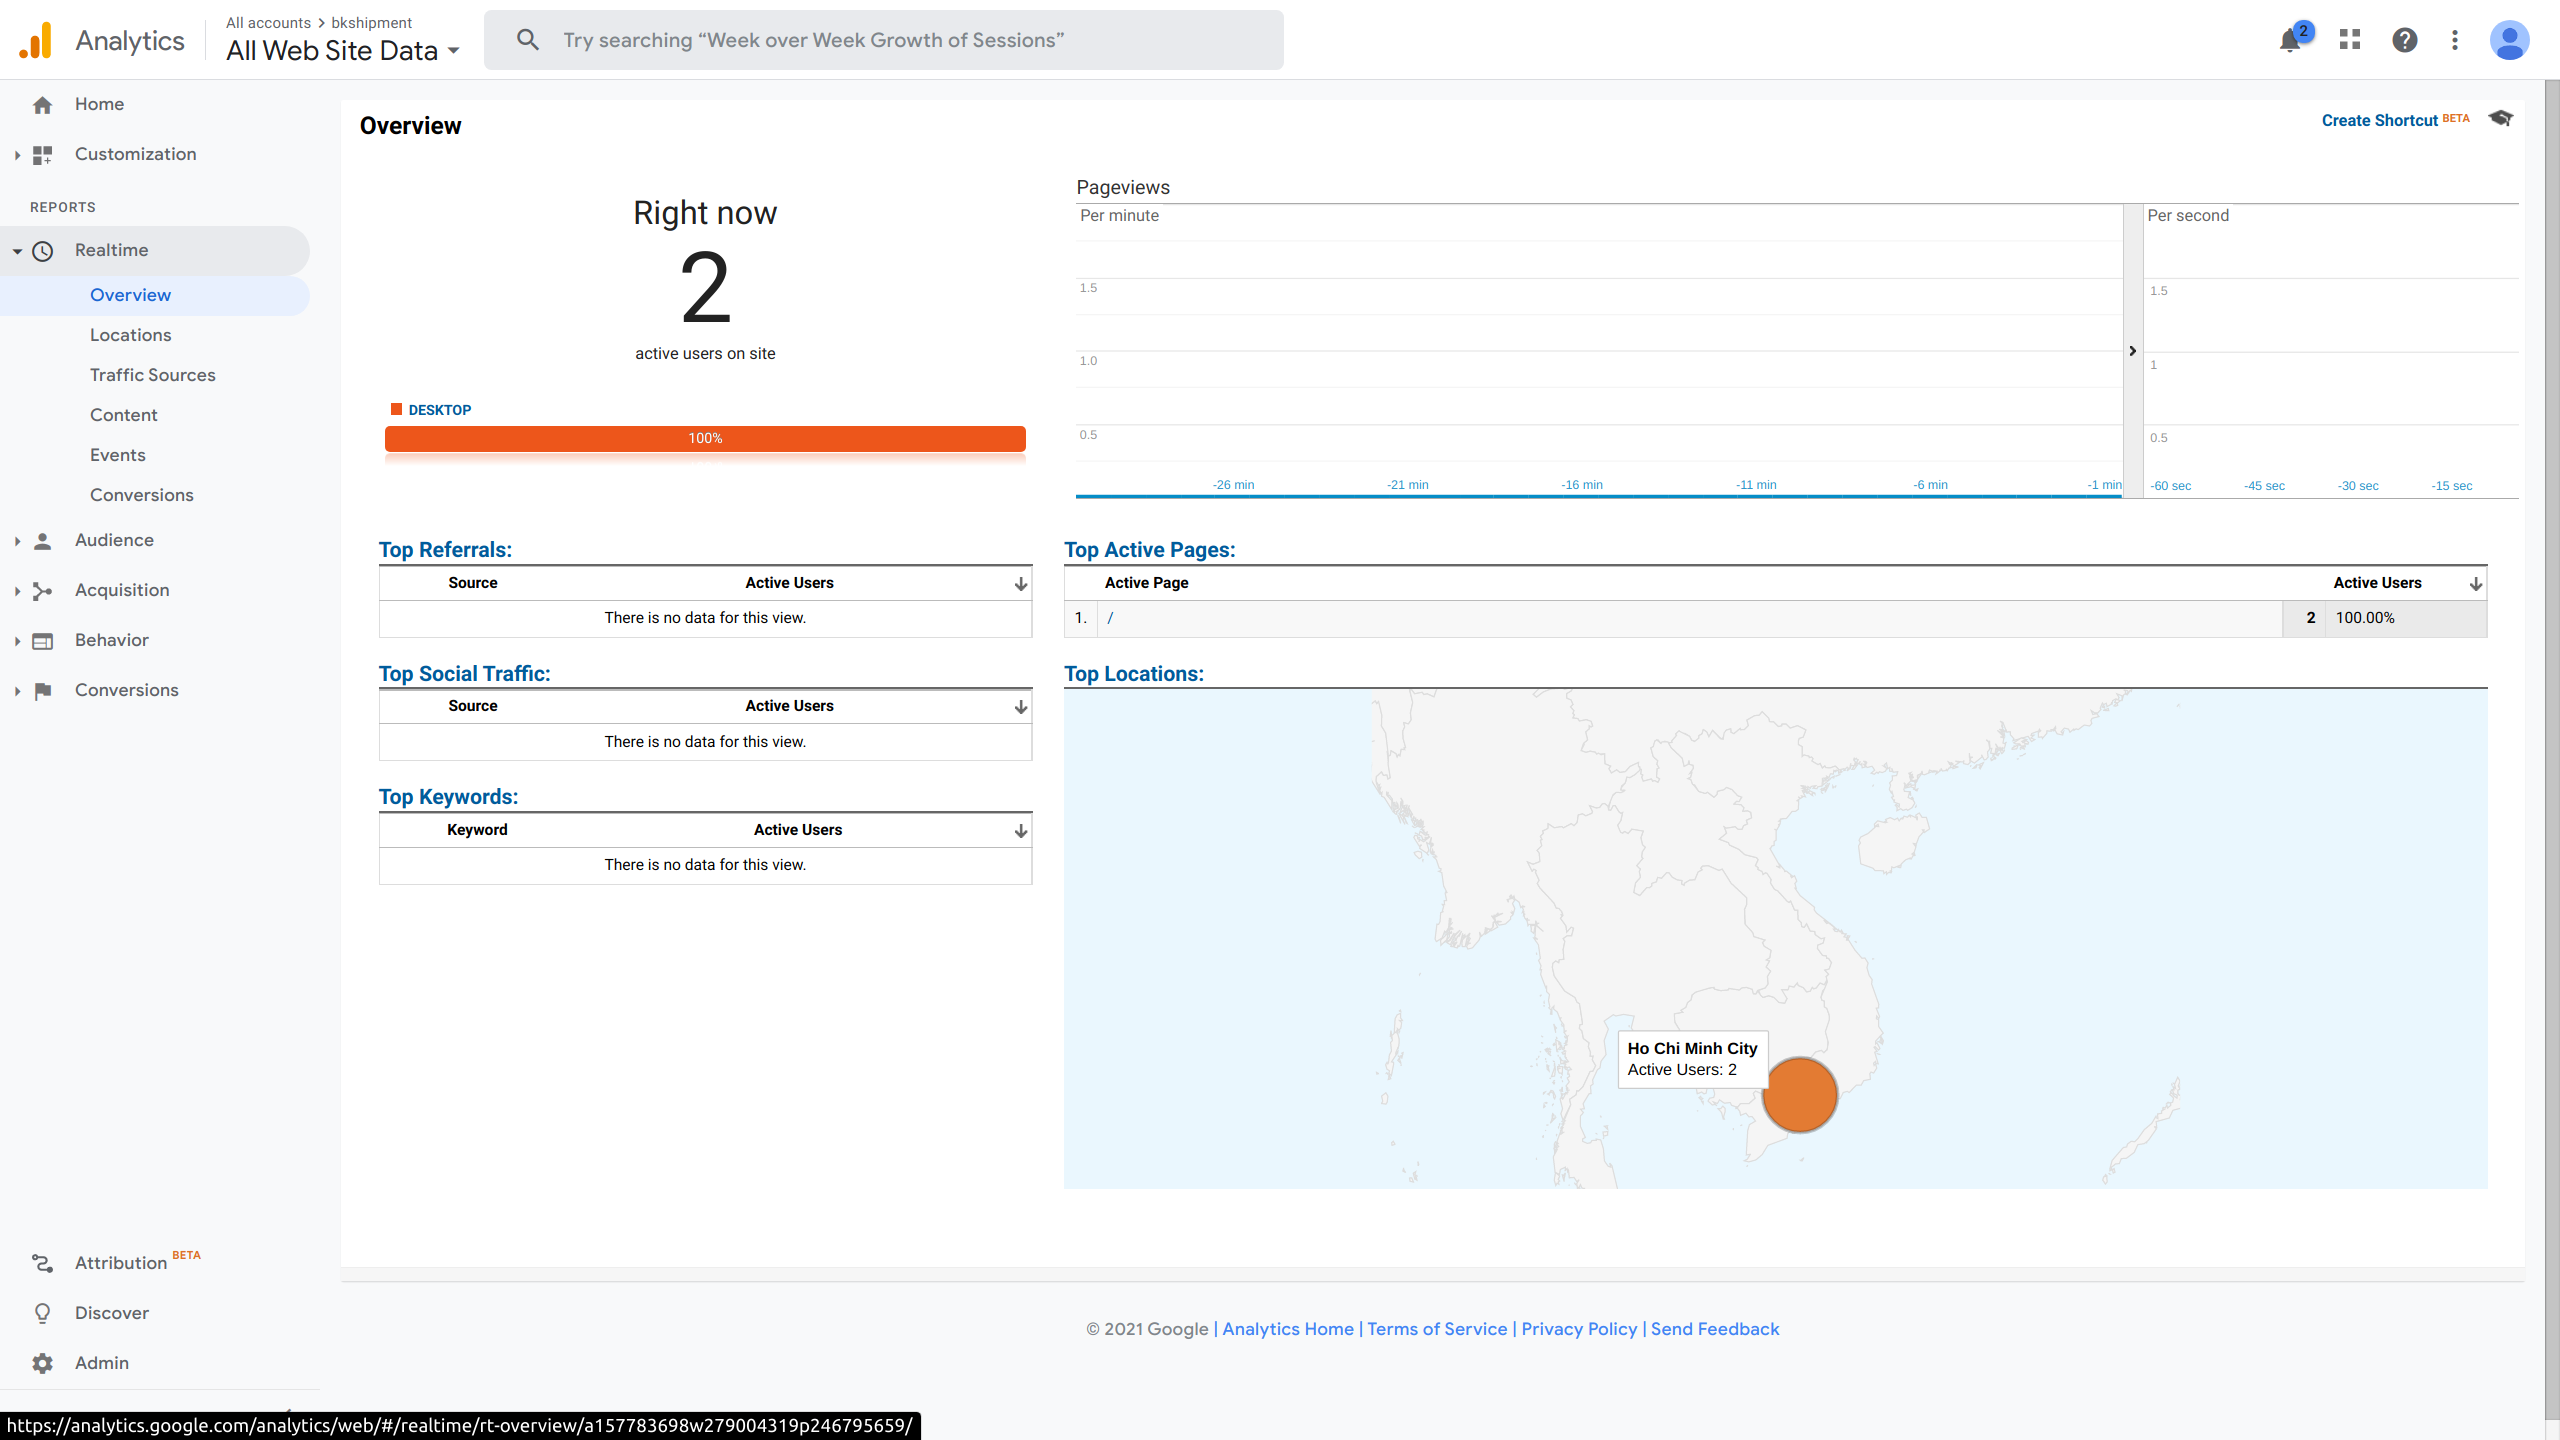
\includegraphics[width=0.8\textwidth]{/GA/GA_overview.png}
			 		\centering
			 		\caption{Màn hình thống kê thời gian thực tổng quan}
			 	\end{figure}
			 	
			 	\begin{figure}[H]
			 		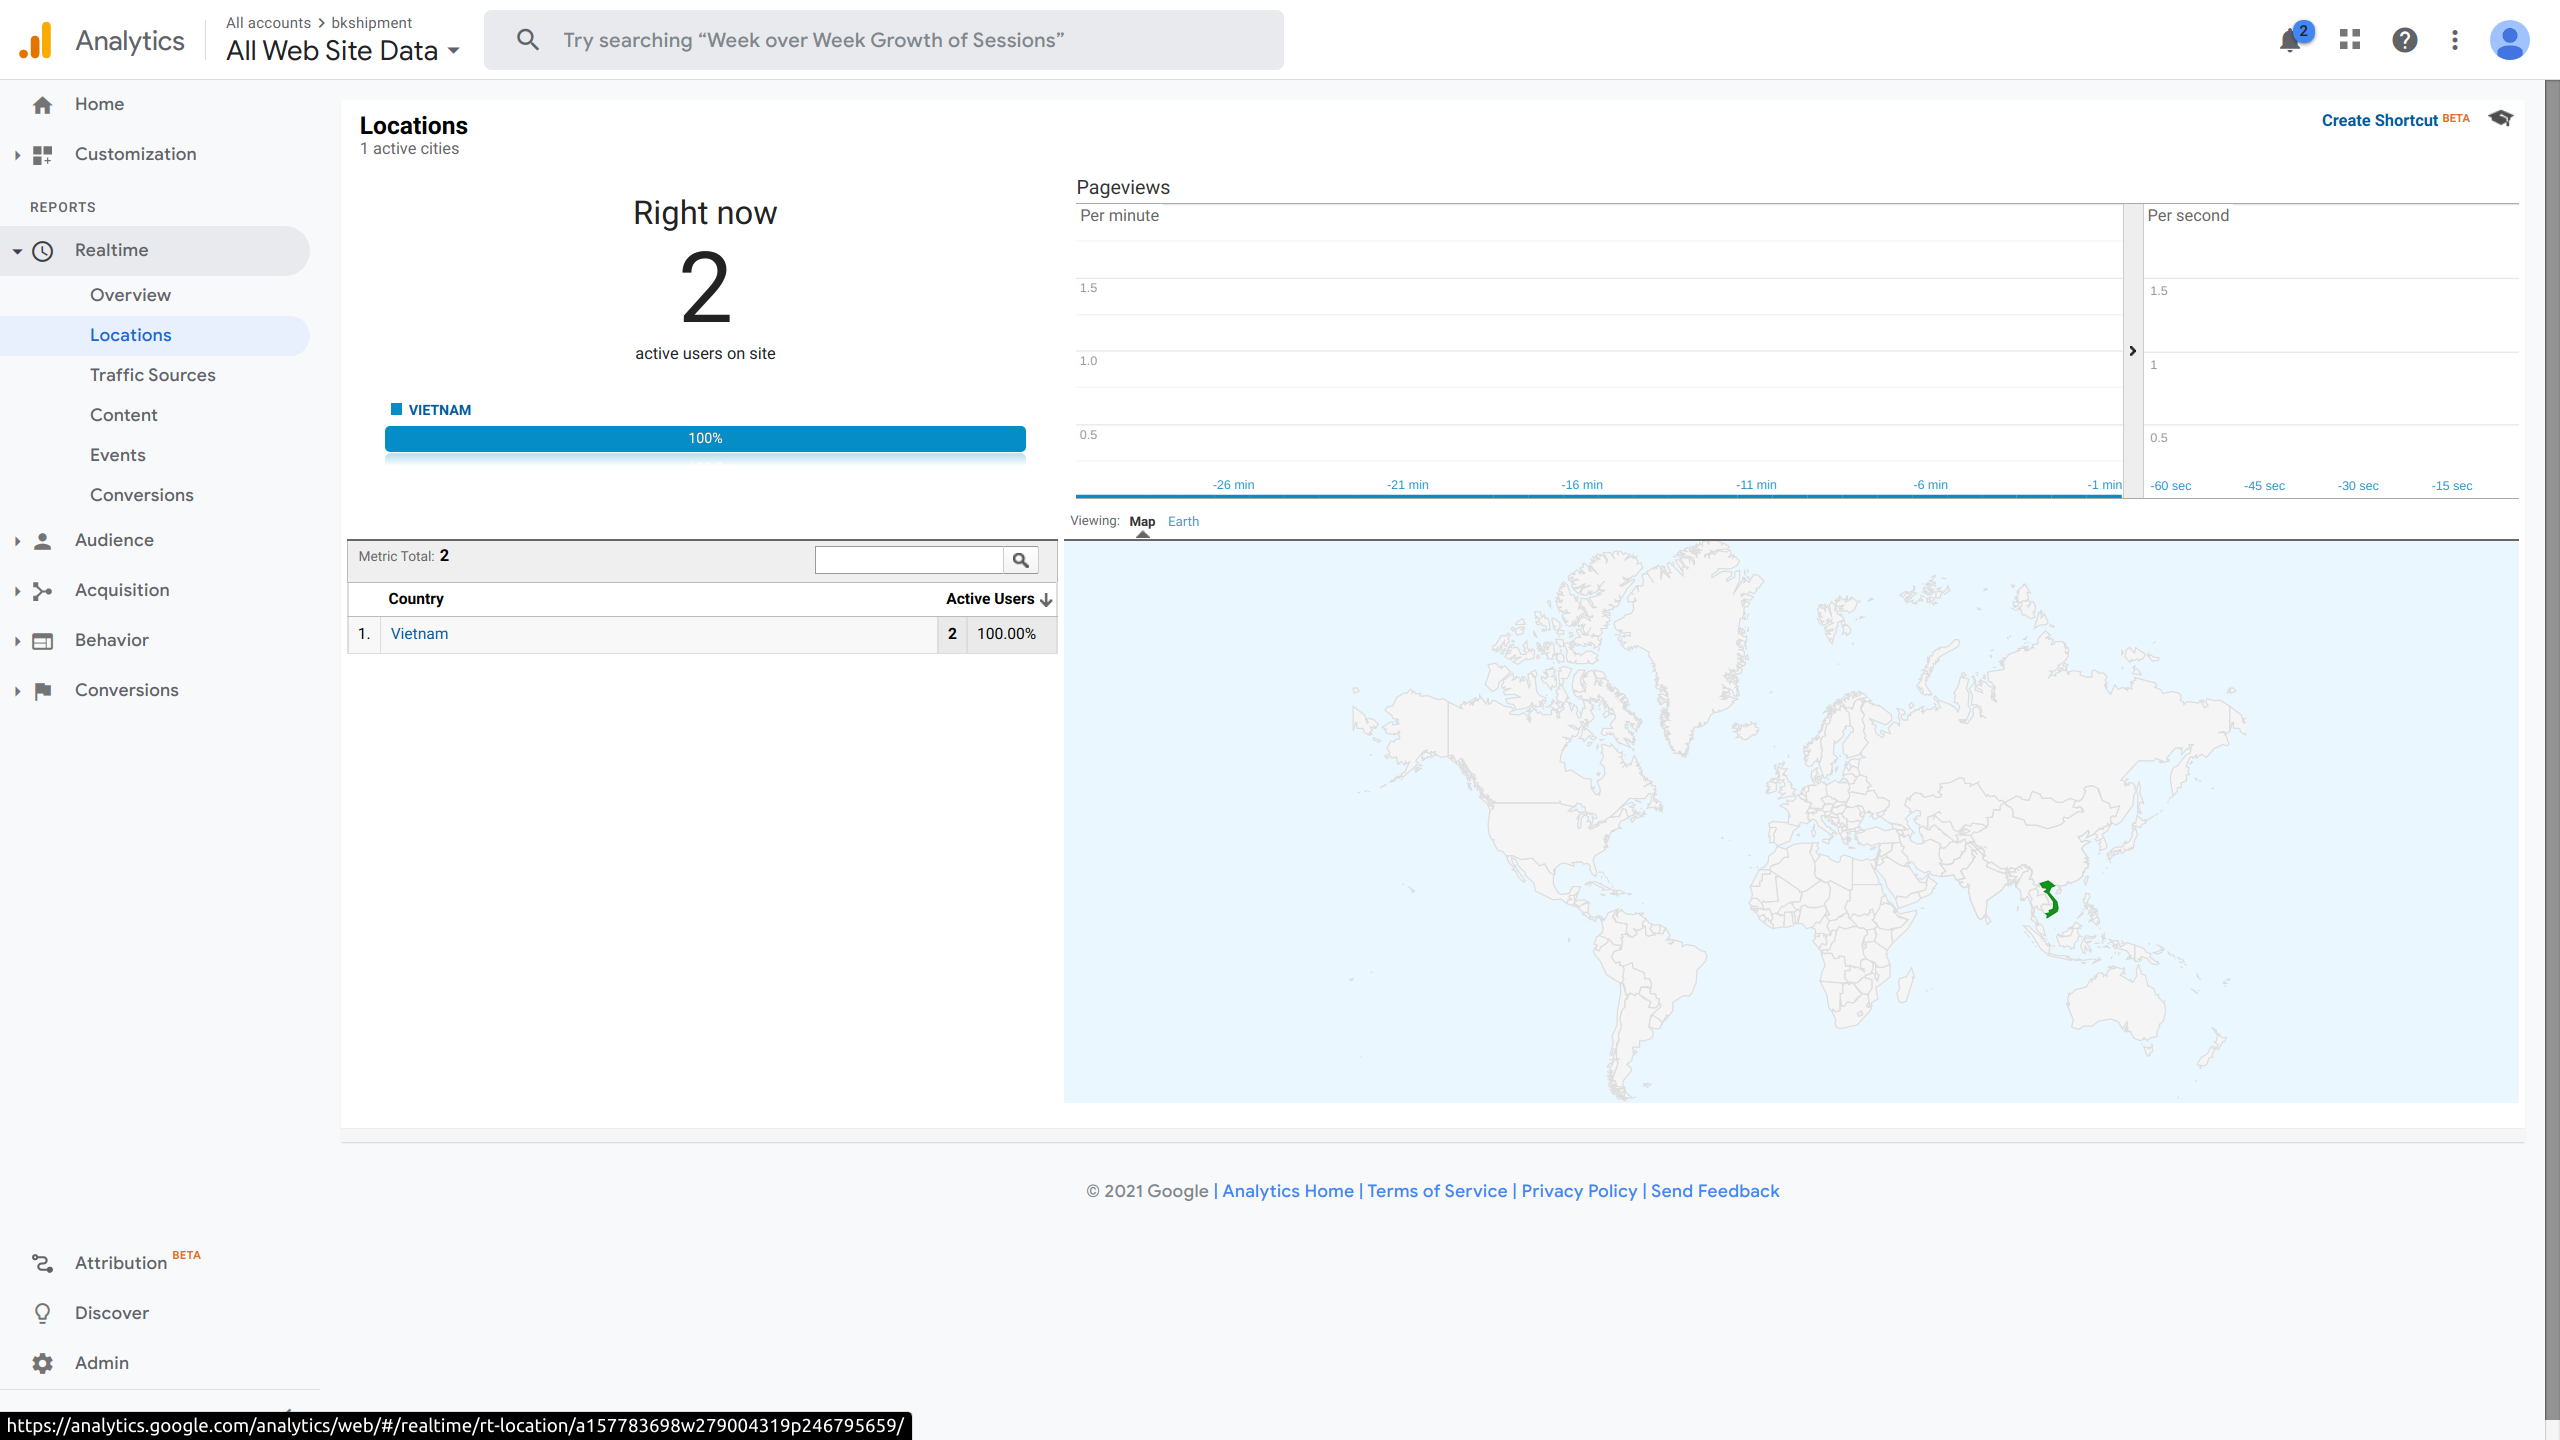
\includegraphics[width=0.8\textwidth]{/GA/GA_location.png}
			 		\centering
			 		\caption{Màn hình thống kê thời gian thực theo địa lý}
			 	\end{figure}
			 	
			 	\begin{figure}[H]
			 		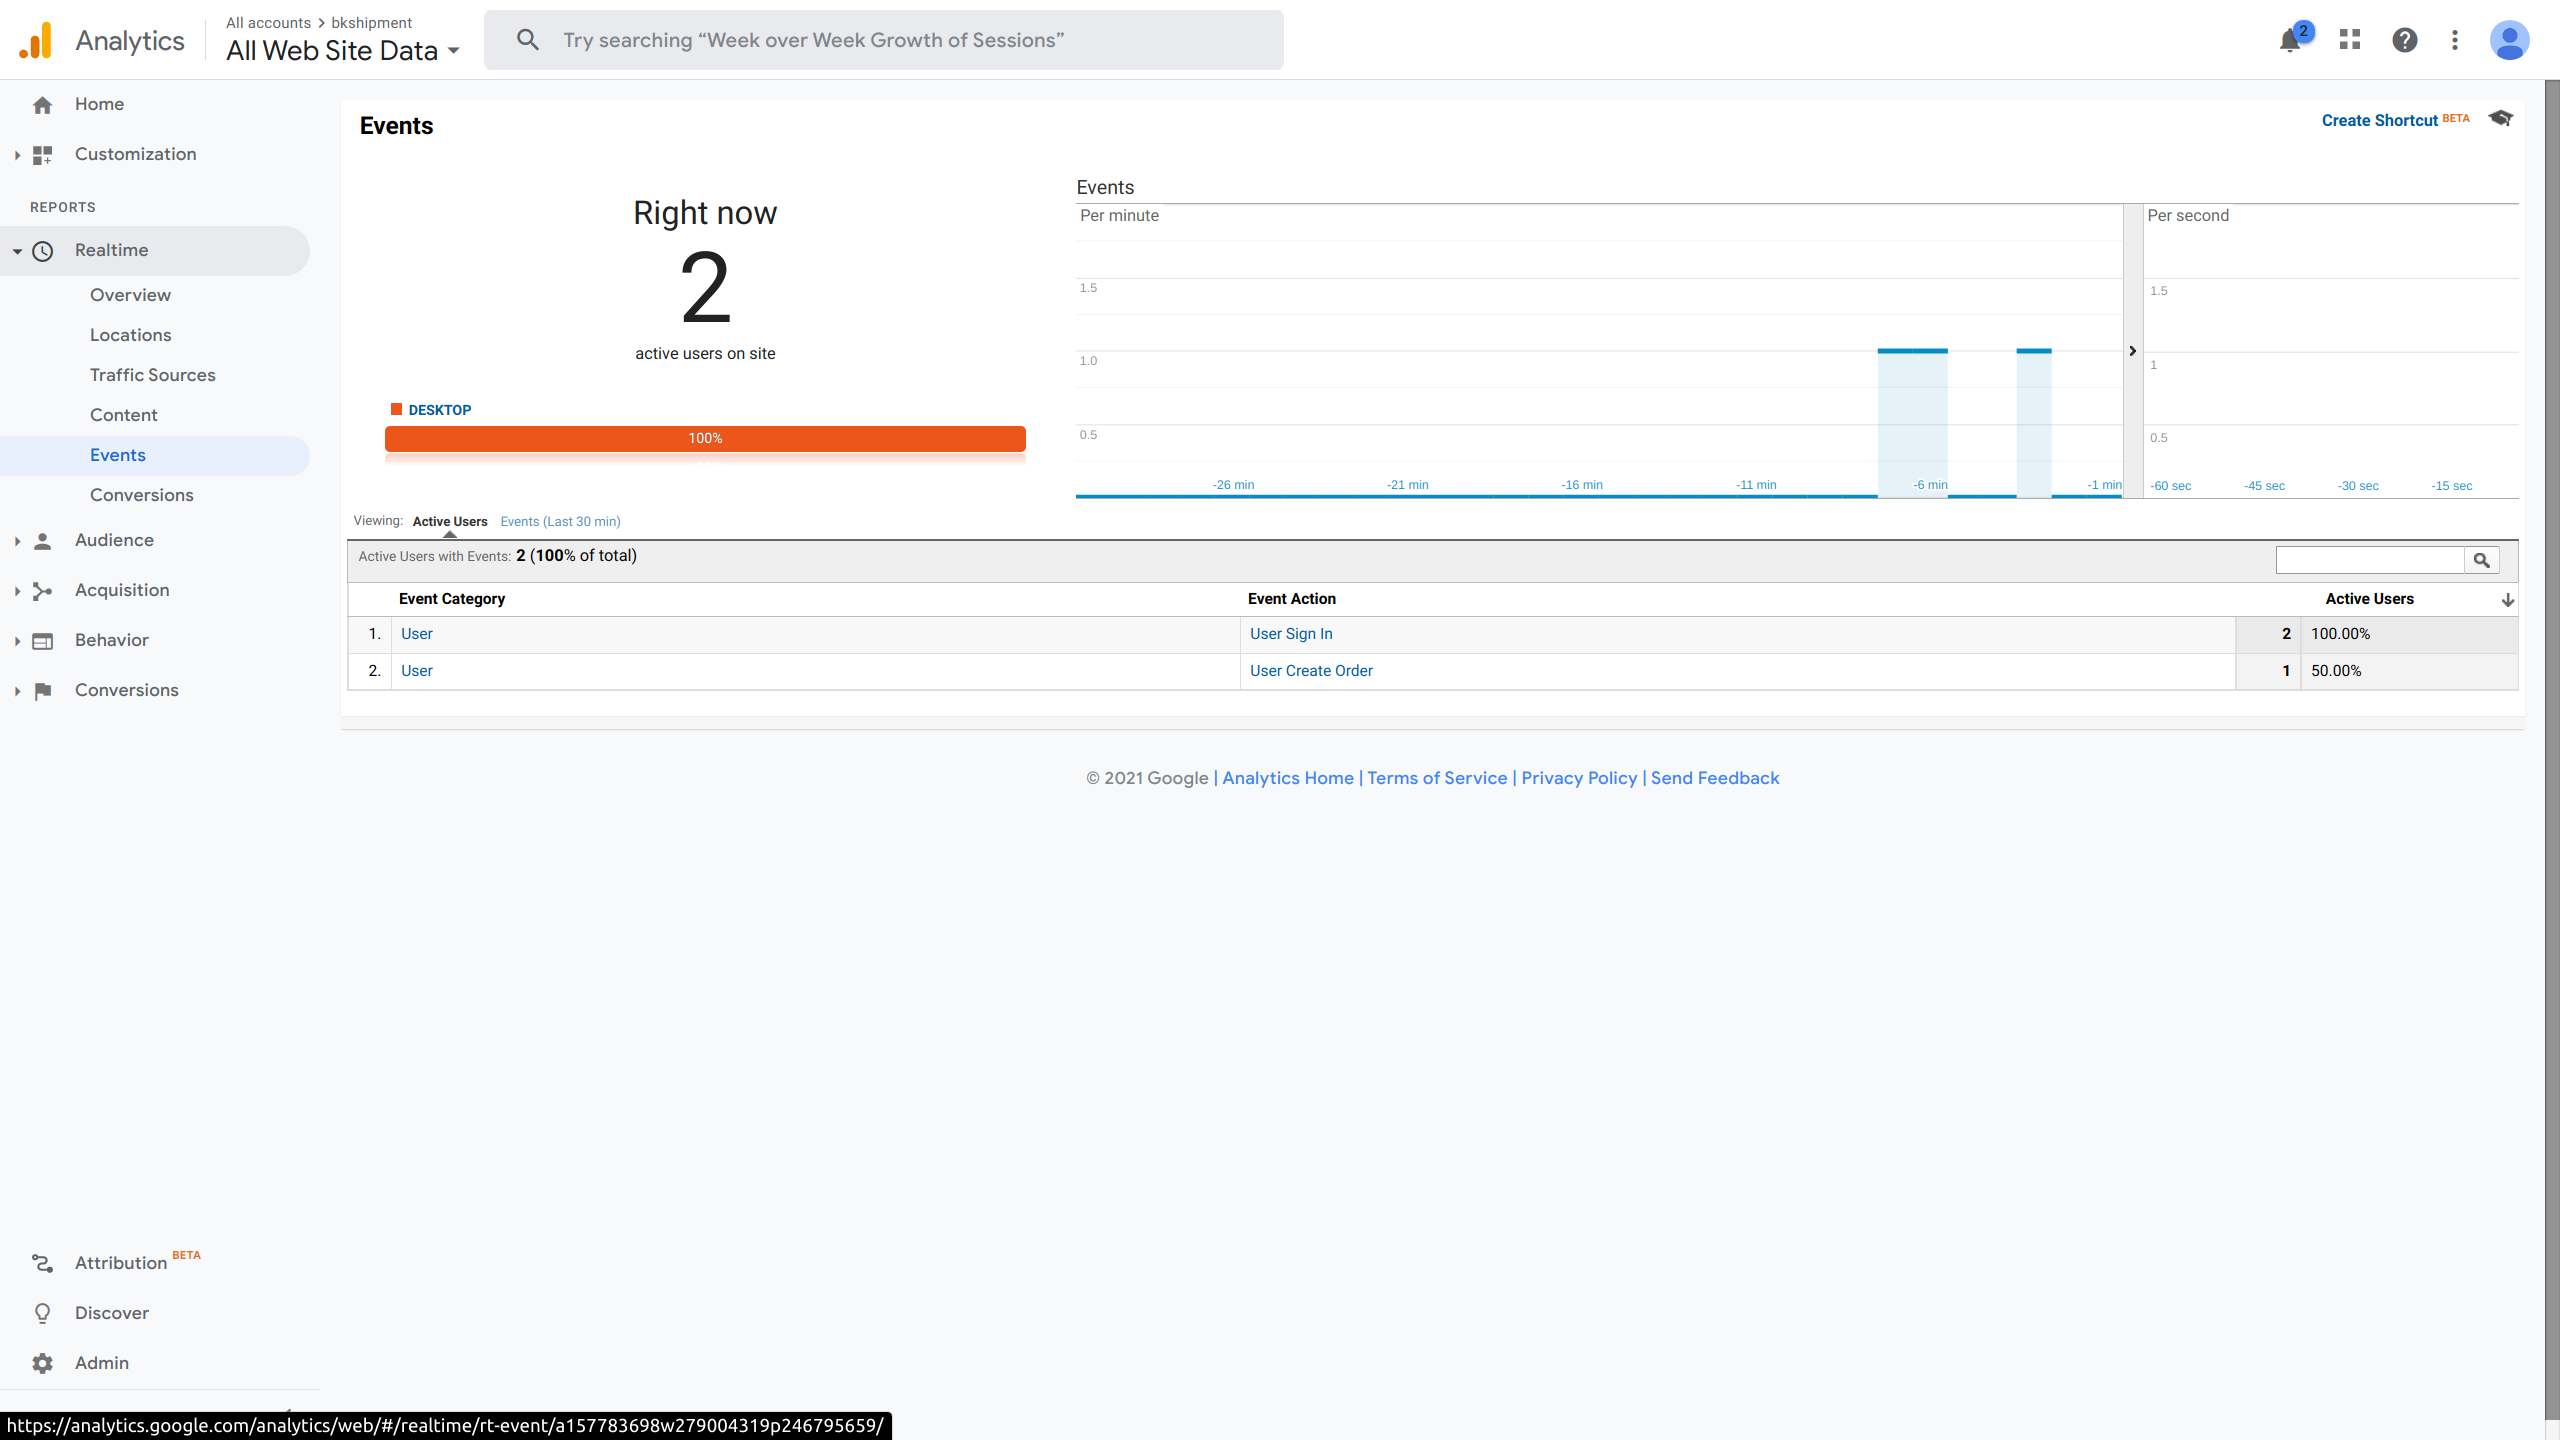
\includegraphics[width=0.8\textwidth]{/GA/GA_events.png}
			 		\centering
			 		\caption{Màn hình thống kê thời gian thực theo sự kiện}
			 	\end{figure}
			 	
			 	Ở các màn hình kể trên, ta đều có thể thấy số lượng người dùng đang truy cập website hiện tại (Ở ví dụ trong hình là 2). Google Analytics cũng giúp chúng ta thống kê người truy cập là ở những nước nào (Ví dụ trong hình là ở Việt Nam) và thống kê những tác vụ mà người dùng thực hiện (Ở ví dụ trong hình ta có thể thấy có 2 tác vụ là người dùng đăng nhập và người dùng tạo yêu cầu gửi hàng). Nhờ những thống kê trên mà đội ngũ phát triển hệ thống có thể đưa ra những quyết định phát triển cho tương lai phù hợp hơn.
			 	
			 	\subsection{Front-end Unit testing}
			 	Trong quá trình xây dựng phần mềm thì việc đảm bảo chất lượng và qui trình kiểm thử phần mềm cũng là một công đoạn rất quan trọng. Không có phần mềm nào là không có lỗi. Chính vì vậy, việc kiểm thử phần mềm giúp hạn chế tối đa lỗi trước khi đưa phần mềm cho khách hàng. Đương nhiên, ngoài đội ngũ xây dựng và phát triển phần mềm cũng cần một đội ngũ tester đảm bảo chất lượng sản phẩm. Tuy vậy, không có nghĩa là lập trình viên chỉ việc viết mã nguồn mà không phải thực hiện kiểm thử phần mềm. Lập trình viên ít nhất cũng nên viết kiểm thử đơn vị (Unit Test) để đảm bảo module mình viết ra ít lỗi nhất có thể và khi có sự thay đổi trong tương lai thì đảm bảo không gây lỗi cho các thành phần cũ của phần mềm.
			 	
			 	\subsubsection{Khái niệm về Unit Test}
			 	Unit Test là một loại kiểm thử phần mềm trong đó các đơn vị hay thành phần riêng lẻ của phần mềm được kiểm thử. Kiểm thử đơn vị được thực hiện trong quá trình phát triển ứng dụng. Mục tiêu của kiểm thử đơn vị là cô lập một phần code và xác minh tính chính xác của đơn vị đó.
			 	
			 	\subsubsection{Lợi ích và đánh đổi của Unit Test}
			 	Thông thường, ở một vài qui trình phát triển phần mềm, đội ngũ kiểm thử phần mềm sẽ yêu cầu lập trình viên phải thực hiện Sanity Test (Kiểm thử sơ bộ) để chắc chắn rằng những những chức năng chính của phần mềm hoạt động ổn định. Mỗi lần sanity test thường có từ vài chục cho đến vài trăm test case và những test case đó có thể xuất hiện lại sau mỗi bản cập nhật phần mềm. Việc phải kiểm đi kiểm lại những test case đó là điều cần thiết, tuy vậy nó khá tốn thời gian và nhàm chán. Chính vì vậy, nếu có thể viết unit test cho những test case đơn giản đó một cách tự động thì sẽ tiết kiệm được rất nhiều thời gian và đảm bảo tính chính xác nếu unit test của người lập trình viết ra có chất lượng tốt. Không những vậy, việc viết unit test sẽ giúp cho người lập trình cảm thấy tự tin hơn mỗi khi xây dựng một module mới hay chỉnh sửa module cũ. Nhờ vào những test case đã viết sẵn đó mà ta có thể chắc chắn sẽ không có lỗi liên quan xảy ra.\\
			 	
			 	Tuy rằng việc viết unit test có rất nhiều lợi ích nhưng có cũng những đánh đổi sau:
			 	\begin{itemize}
			 		\item Tốn thời gian và tương đối khó khăn. Viết test tuy giảm bớt thời gian và công sức cho giai đoạn duy trì (maintain) phần mềm nhưng sẽ làm mất thời gian lúc đầu để viết một unit test tốt.
			 		\item Test pass không có nghĩa ứng dụng, function của chúng ta chạy đúng hoàn toàn.
			 		\item Cũng đôi khi, test fail, nhưng ứng dụng, function vẫn chạy hoàn toàn bình thường. Việc viết test không tốt như vậy sẽ còn nguy hiểm hơn do nó tạo cho người lập trình một suy nghĩ rằng phần mềm viết ra không có lỗi, trong khi thực sự thì có.
			 	\end{itemize}
			 	
			 	\subsubsection{Viết unit test cho client-side code của hệ thống}
			 	Có thể hiểu nôm na, viết unit test cho Front-end thì ngoài viết test cho những hàm tính toán, ta còn có thể viết test để kiểm thử giao diện và hành vi khi một số sự kiện người dùng xảy ra. Chẳng hạn sau đây là một số thứ ta có thể kiểm thử ở client-side code:
			 	
			 	\begin{itemize}
			 		\item Kiểm thử xem một node trong cây DOM có xuất hiện (tồn tại) trong giao diện sau khi đã render component hay chưa. Chẳng hạn kiểm thử xem giao diện đăng nhập có tồn tại một nút với dòng chữ là "Đăng nhập" hay không. Hay nút đó có được áp dụng đúng class hay không để có style css đúng như mong muốn.
			 		\item Kiểm thử xem sau khi người dùng đã nhập đủ thông tin đăng nhập và ấn nút đăng nhập, người dùng có chuyển đến trang màn hình chính hay không.
			 		\item Chẳng hạn giao diện ta có một carousel có yêu cầu cứ mỗi 2 giây sẽ chuyển sang hình kế tiếp. Ta có thể viết unit test để kiểm chứng điều đó.
			 	\end{itemize}
			 	
			 	Trên đây chỉ là một số ví dụ về những chức năng ta có thể thực hiện bằng việc viết unit test cho front-end code của ứng dụng.\\
			 	
			 	Nhóm sẽ ví dụ 2 test case đơn giản mà nhóm đã viết để demo việc áp dụng việc viết unit test vào hệ thống. Nhóm sẽ dùng 2 thư viện hỗ trợ cho việc viết test cho những component của React khá phổ biến hiện nay: \textbf{Jest} và \textbf{React Testing Library}. 2 test case đơn giản mà nhóm sẽ viết sẽ như nhau:
			 	
			 	\begin{itemize}
			 		\item Kiểm thử xem component để hiển thị khi data rỗng có dòng chữ \textbf{Không có dữ liệu hiển thị} tồn tại trong giao diện nếu component được render hay không.
			 		\item Kiểm thử xem component hiển thị data rỗng đó có hiển thị hình ảnh đi kèm mong muốn hay không.
			 	\end{itemize}
			 	
			 	\begin{figure}[H]
			 		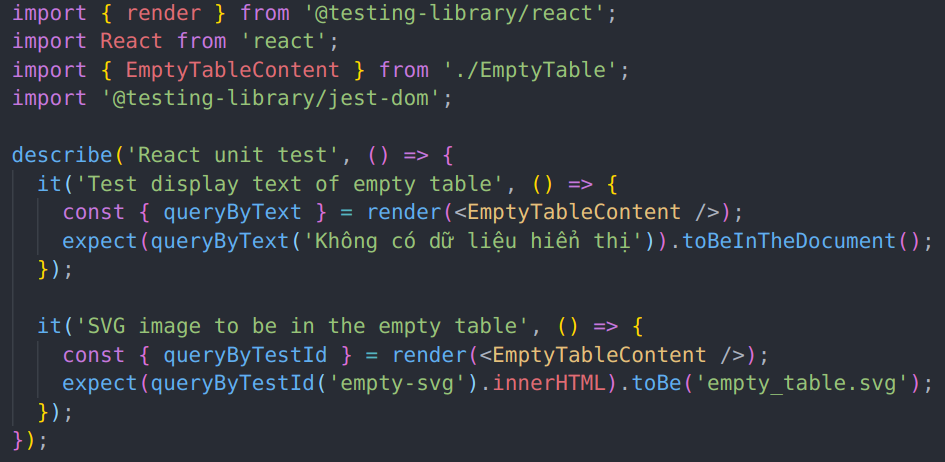
\includegraphics[width=0.8\textwidth]{/FE_unit_test/code.png}
			 		\centering
			 		\caption{Đoạn mã hiện thực}
			 	\end{figure}
			 	
			 	\begin{figure}[H]
			 		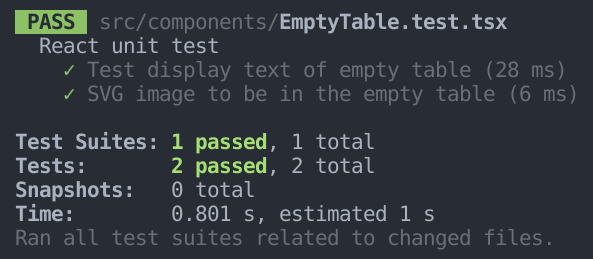
\includegraphics[width=0.8\textwidth]{/FE_unit_test/result.png}
			 		\centering
			 		\caption{Kết quả chạy 2 test case}
			 	\end{figure}s
			 	
			 	\subsection{Tổng kết}
			 	Trên đây là những công nghệ nhóm đã dùng để hiện thực tương đối hoàn chỉnh phần front-end của hệ thống. Một hệ thống Front-end hoàn chỉnh không những chỉ cần những thành phần để hệ thống có thể chạy được mà cần phải có hệ thống track lỗi, thống kê truy cập vào website và đảm bảo lỗi thông qua unit test.
		
	